% arara: pdflatex: { synctex: on, interaction: nonstopmode, shell: yes }
% arara: pdflatex: { synctex: on, interaction: nonstopmode, shell: yes }

\documentclass[hidelinks]{article}

\usepackage[utf8]{inputenc}
\usepackage{graphicx}
\usepackage{caption}
\usepackage[svgnames]{xcolor} % for 'lightgray' color
\usepackage{hyperref}
\usepackage{listings}

\graphicspath{ {./} }

\newcommand{\code}[1]{\colorbox{lightgray}{\texttt{#1}}}

\title{Circular Track System Documentation}
\author{Ghassan Arnouk \& David Song}
\date{\today}

\begin{document}

\maketitle
\clearpage

\tableofcontents
\clearpage

\listoffigures
\clearpage

\lstlistoflistings
\clearpage

\section{Introduction}
The circular track system is currently being used to test a variety of surfaces and their response to EM excitation in the X-Band (8-12 GHz). It consists of 3 main components, the Agilent 8720ES Vector Network Analyzer (VNA) and associated antennae apparatus, the rotary stage, and associated control apparatus, and finally the National Instruments (NI) PXIe-1071 Modular Instrumentation body. The 3 components will be discussed in further detail below.
\clearpage
\section{System Overview}
\begin{center}
    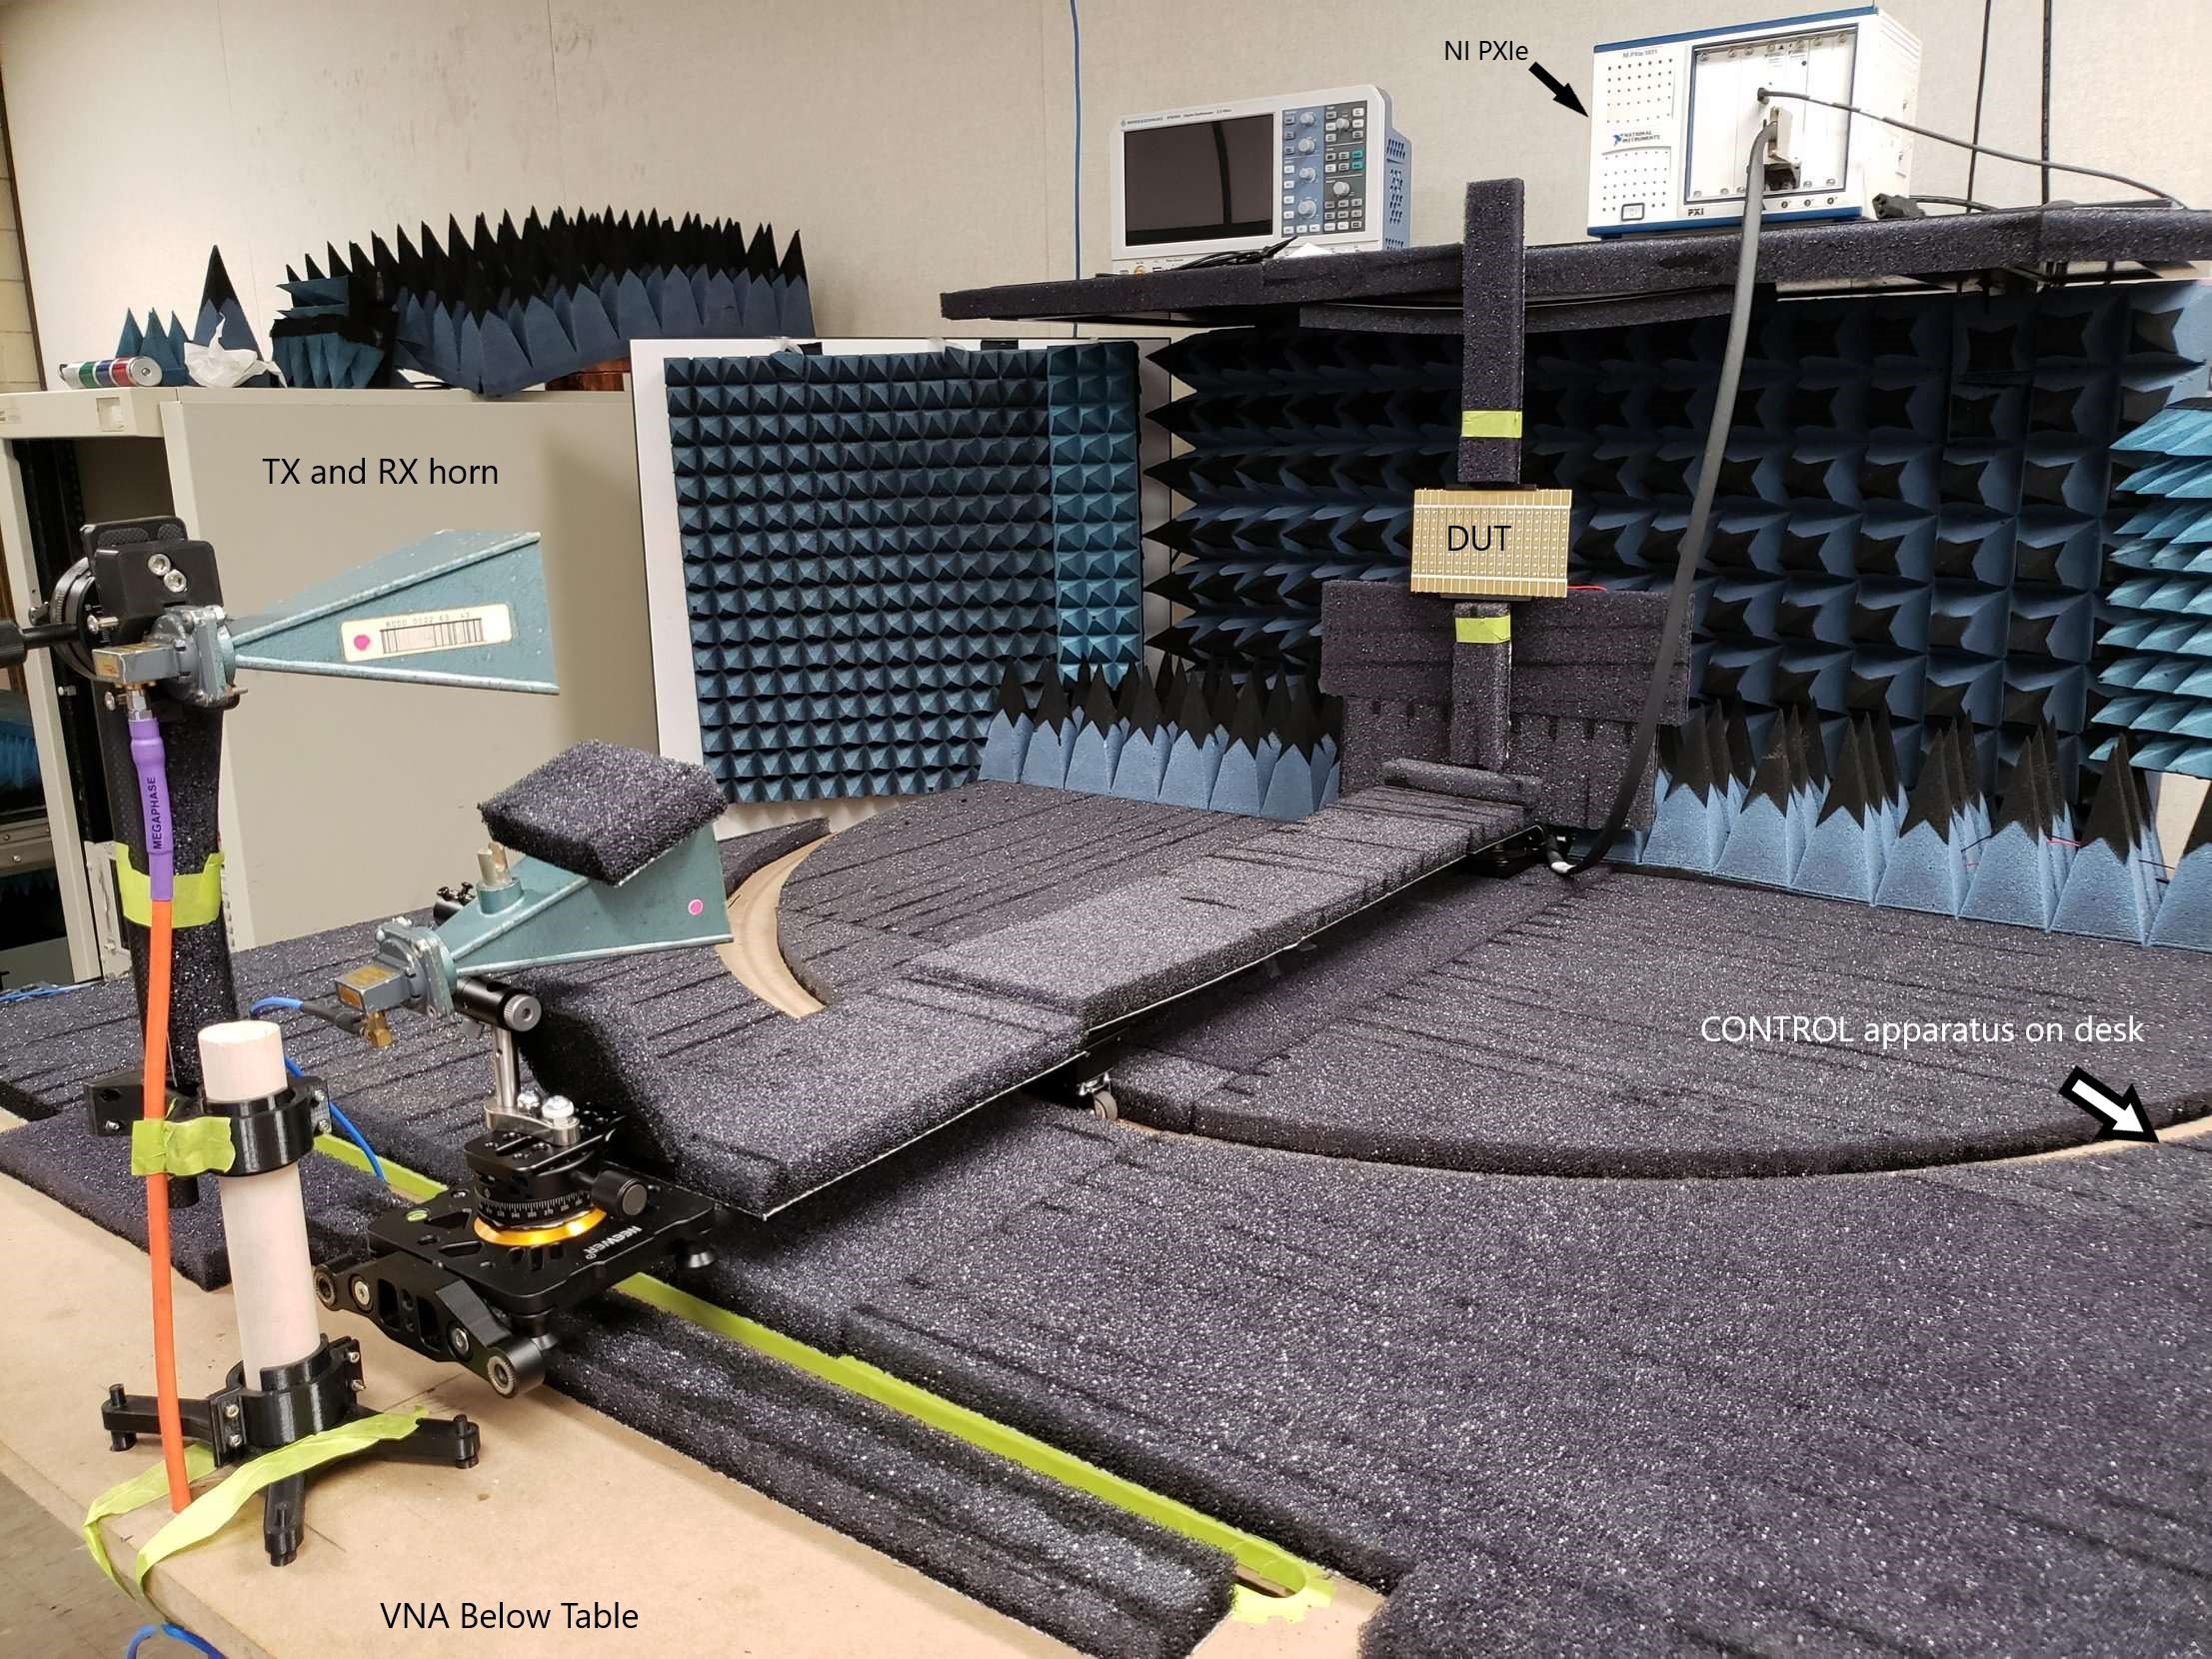
\includegraphics[width=\textwidth]{annotated_figure.jpg}
    \captionof{figure}{System setup diagram}
\end{center}
The setup is shown below, With a DUT set up on the stand. The locations of the major components are indicated

\section{Installation}
This section outlines the installation, and update of the package. We cannot assume that the computer in the nearfield room will always have the script locally available. 

\subsection{cloning the Github repository and installing commands}
The Github repository can be cloned either through Github gui, Git CLI or simply downloading the zip file from the Github page. It can be accessed at the following link: \href{https://github.com/kgein/MARS-CircularTrackSystem}{\textcolor{blue}{MARS REPO}}. please contact Keigan MacDonell for access to the repository (). When the folder is in the appropriate directory, run the following command in the command prompt opened using anaconda navigator: either open it from anaconda navigator or the start menu:
\begin{center}
    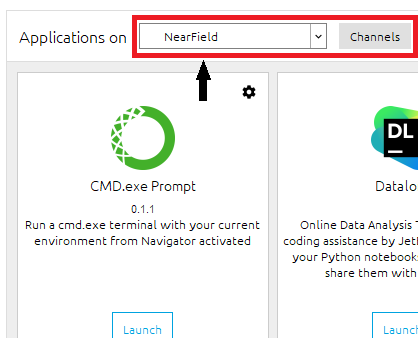
\includegraphics[width=0.5\textwidth]{asdasda.png}
    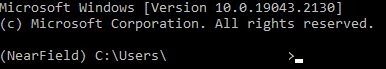
\includegraphics[width=0.5\textwidth]{asdasdaaffwaf.png}
\end{center}
Ensure that the environment is set as above, ie. you are working inside the nearfield environement, then run the following code: \\\\\code{pip install --editable .}\\\\
The ctrack script and all dependencies are now installed

\section{QuickStart}
This section will detail how to quickly get set up to take an angle sweep measurement from -70 to 70 degrees around the surface. The PXIe is not used in this case

\subsection{Preparing Setup}
Firstly ensure that the VNA has been on for at least one hour before taking measurements. This is to ensure that the VNA has warmed up to give the most accurate results. The BBBBB or AAAAA calibration can be used, or it is highly recommended to re-calibrate if any of the connectors or cables have changed.\\

Ensure that all the connections are plugged in as follows:\\
\begin{itemize}
    \item VNA is plugged in and on, and the GPIB connector is plugged into the computer's USB port
    \item Ensure both TX and RX horns have the coaxial cables connected tightly with the proper torque setting (0.9 Nm)
    \item Ensure that that the power supply is plugged in and connected to the motor controller board.
    \item Ensure Arduino is plugged into the computer USB port
\end{itemize}
\subsection{Aligning horn and Surface}
When all connections are properly made, power on all apparatus. Align the the horns using the laser apparatus, as shown below:
\begin{center}
    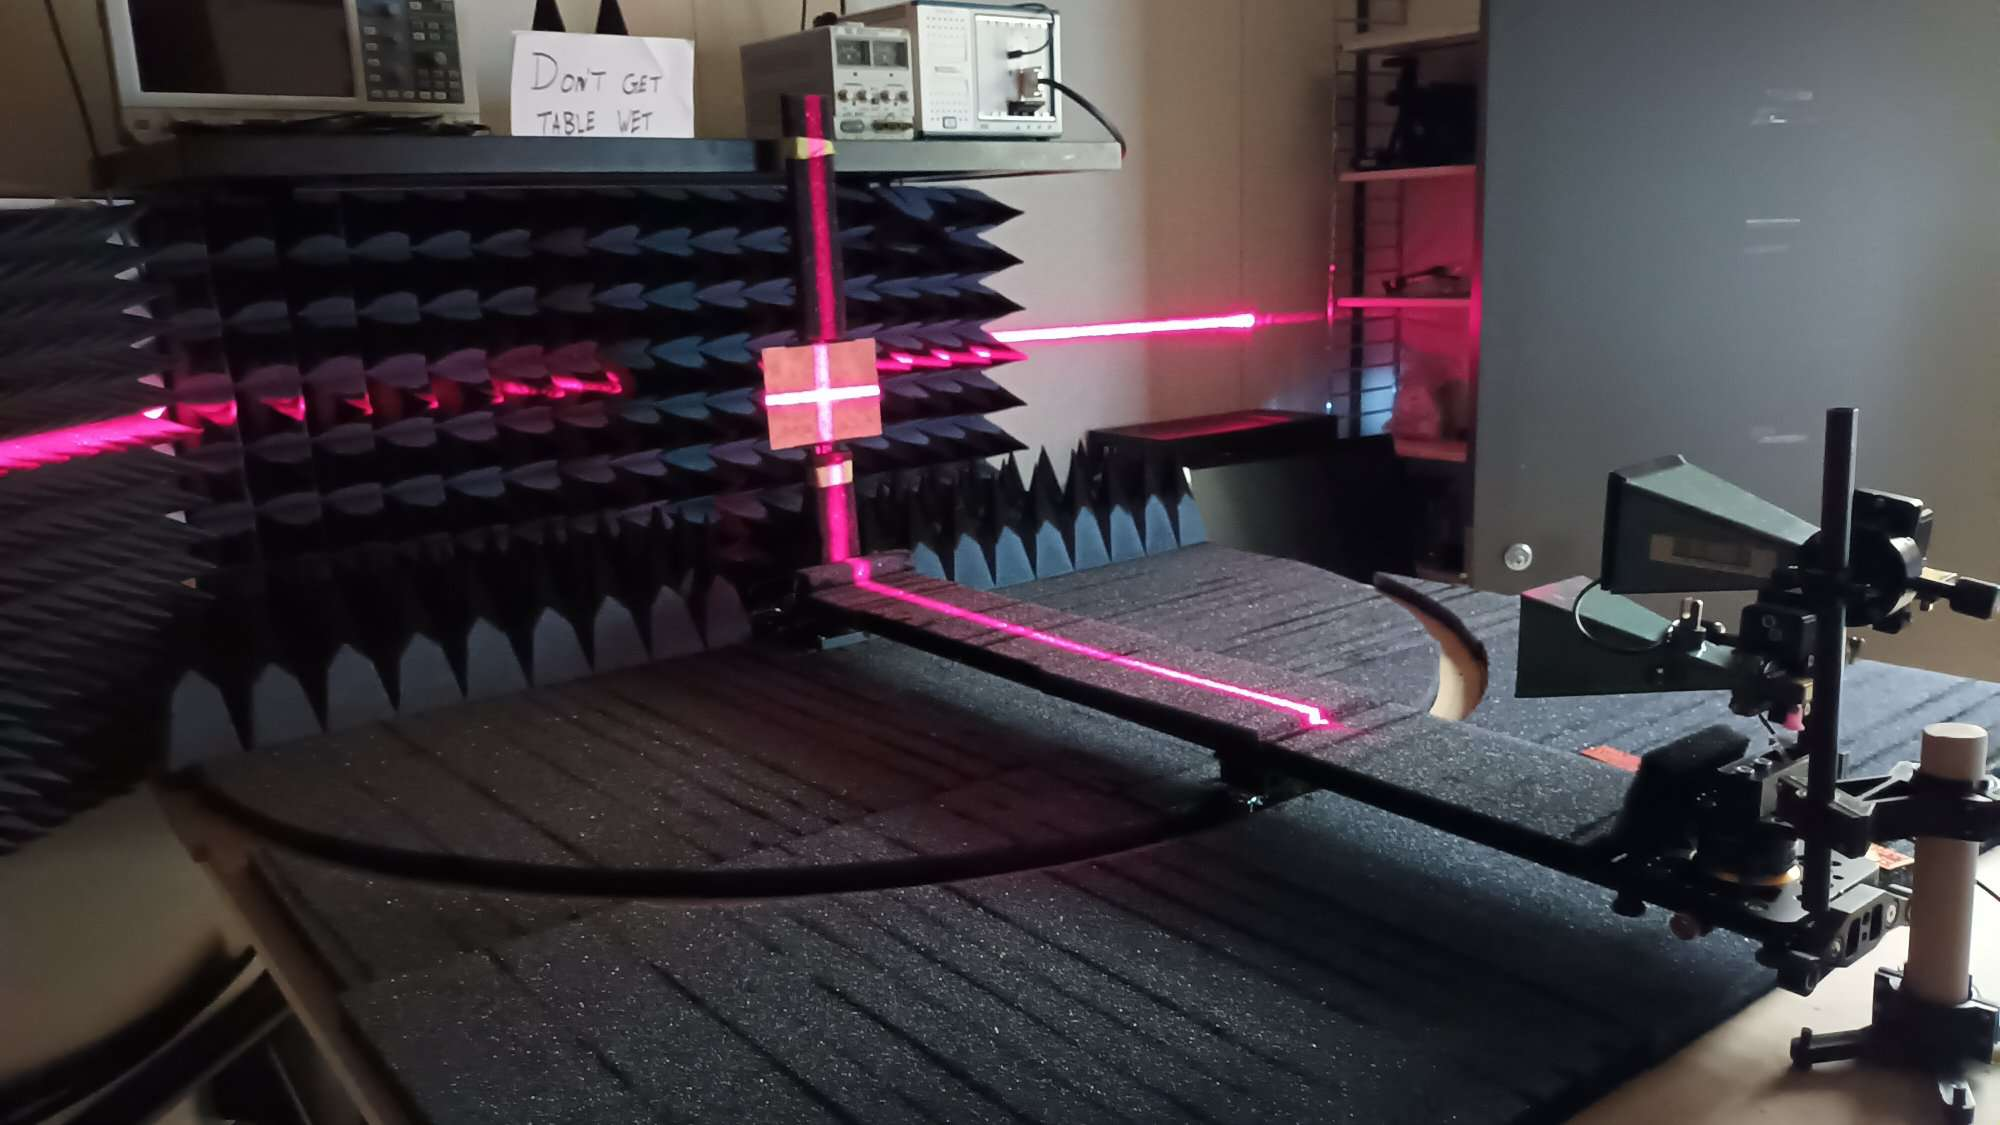
\includegraphics[width=\textwidth]{imgpsh_fullsize_anim (1).jpg}
    \captionof{figure}{Alignment of horns using a laser level}
\end{center}
The stand uses elastics to hold the surface securely in place. Ensure that the notches accept the edge of the surface to ensure a zero degree incident angle at the resting position. The stand indexes into a notch in the rotary stage, so do not force the stand into position, it will only fit in one direction.
\subsection{Performing Measurement}
Navigate to the desired save directory, and create a folder called \code{cli\_measurements}. This is done to avoid overwriting previous data, and to ensure that the user knows where the saved data is \\
When the horns are level, the arm may be moved to the -70 degree location (Clockwise from the original resting position) using the following command:
\begin{center}
    \code{ctrack rotate -d 70 l}
\end{center}
This will move the arm to 70 degrees clockwise position. The sweep will start when the following command is executed. The 
\code{-n} option allows you to specify the name of the sweep, as seen below, replacing \code{name} with the desired name. The command will autogenerate a directory structure to save the results as long as the \code{cli\_measurements} folder is present, but this can be overwritten if needed with a \code{-p} command.
\begin{center}
    \code{ctrack asweep -a -70 70 -s 0.5 -n name}
\end{center}
This will begin a sweep from -70 degrees to 70 degrees consisting of a 140 degree arc, with 280 distinct data points (a 0.5 degree sweep increment).\\
The sweep will take about 10 minutes to complete, after which the results are output as a CSV file which can be used as desired for further data processing.
\clearpage
\section{General Information}
\subsection{script location and commands}
The script is currently located at:\\ \code{C/Users/keiganmacdonell/OneDrive - Carleton University/REPOS/}\\\code{MARS-CircularTrackSystem/old/templates/python/may13}. \\
It is backed up as well to github. One does not need to be in this directory to run the scripts, the only requirement is to create a folder called \code{cli\_measurements} in the current CMD promt directory\\

The following is a comprehensive list of all commands currently implemented in the script. The whole script is modular and uses shallow wrapper functions to excecute the underlying code, using the click python library:
\subsubsection{getfreq}
This command returns a FreqSweepParams object with the frequency sweep start, end, number of points, power and averaging. It will also print the information to the console screen.
\\\\\textbf{Use}\\
\code{ctrack getfreq}\\\\
\textbf{Expected output example}\\
\code{start:8.000E+09 stop:1.200E+10 points:201 power:-10.00 averaging:1}
\subsubsection{setfreq}
This command will allow a user to specifiy the start and end frequencies (specify in GHz, conversion is automatic) and the number of points. If an invalid entry is performed, the VNA will default to a specific value. The following will set a frequency sweep from 8 GHz to 12 GHz with 1601 points.
\\\\\textbf{Use}\\
\code{ctrack setfreq -s 8 -e 12 -p 1601}\\\\
\textbf{Expected output example}\\
This command produces no output, but the results can be easily checked with a \code{getfreq} command
\subsubsection{setpwr}
This command allows a user to specify the power in dB for the sweep, from +5 to -80 dB
\\\\Use:\\
\code{ctrack setpwr -p -10}\\\\
\textbf{Expected output example}\\
No output but can be again checked as above.
\subsubsection{rotate}
This command allows the user to quickly rotate the arm a desired number of degrees clockwise or counterclockwise. The frame of reference is facing the stage from the end of the table. A `l' or `r' at the end of the command denotes the direction (l = cw, r = ccw)
\\\\\textbf{Use}\\
\code{ctrack rotate -d 70 l}\\\\
\textbf{Expected output example}\\
The arm will rotate as long as the power supply is on
\subsubsection{display4}
This command switches the VNA display to a 4 window display with all S parameters shown.
\\\\\textbf{Use}\\
\code{ctrack display4}\\\\
\subsubsection{asweep}
This script runs a sweep of angles from the start location to end location.
\\\\\textbf{use}\\
\code{ctrack asweep -a -70 70 -s 0.5 -n PEC\_0db\_sweep\_2}\\\\
\textbf{Expected output example}\\
Console window will output step feedback and current angle, while arm will move and take measurements. Data is saved in the directory the script is run from in a folder called \code{cli\_measurements}

\subsubsection{fsweep}
This command will perform a stationary sweep at the specified angle
\\\\\textbf{use}\\
\code{ctrack fsweep -a 0 -n PEC\_0db\_sweep\_2}\\\\
\textbf{Expected output example}\\
Will save data in a folder in the directory the script is run from called \code{cli\_measurements}
\subsubsection{nisetall}
This script sets all channels on the NI PXIe module to the given voltage
\\\\\textbf{use}\\
\code{ctrack nisetall -v 2}\\\\
\textbf{Expected output example}\\
Sets all channels on the NI to 2 volts
\subsubsection{nisetone}
This script sets \textbf{one} channel on the NI PXIe module to the given voltage
\\\\\textbf{use}\\
\code{ctrack nisetone -v 2 -c 0}\\\\
\textbf{Expected output example}\\
Sets channel 0 on the NI to 2 volts. One can write a series of commands in a batch file to precisely set all desired channels to the right voltage quickly
\subsubsection{setifbw}
This script sets the IF filter bandwidth to the desired value. The values are discrete and can be set to 10, 30, 100, 300, 1000, 3000, 3700 or 6000 Hz respectively.
\\\\\textbf{use}\\
\code{ctrack setifbw -f 3000}\\\\
\textbf{Expected output example}\\
Sets IF filter BW to 3000 Hz.
\clearpage
\subsection{Rotary Stage}
The rotary stage is a \href{https://www.robotdigg.com/product/1628/PT-GD201-203-and-204-Stepper-Motorized-Electric-Rotary-Table}{\textcolor{blue}{RobotDigg PT-GD201}} driven by a NEMA-17 form factor motor. The motor is a bipolar stepper, with 4 inputs which can be driven by a variety of different controllers. The current motor is capable of handling 1.5 Amps maximum under load. The driver board being used is a MP6500 Stepper Motor Driver Carrier by Pololu but any similar driver can be used such as the DRV8825 that can handle at least 1 amp of current output continuously. The stage is calibrated so that one full revolution of the stepper motor shaft is equivalent to a 2 degree movement of the upper rotating portion of the stage. Thus a conversion factor can be obtained to convert between number of steps and number of degrees (1 degree = 100 steps).\\

The motor system is driven by an arduino uno, as a cheap way to interface the serial commands from the python script to the rotary stage. A breakdown of the entire system is shown below on a breadboard. The actual system is contained inside an enclosure near the setup:
\subsection{Antennae mount}
The antennae are mounted on a set of mounts that allow the variation of the antennae polarization in the x and y directions. The diagrams below show the operation of the mount: 
\subsection{DUT Stand}
The DUT stand is designed to hold planar metasurfaces of various forms
\section{VNA}
The VNA being used is the Agilent 8720ES. It is capable of producing frequencies from 50 MHz to 20 GHz, at a variety of power ranges. Each frequency sweep can consist up to 1601 distinct points. Many of these features can be controlled to a degree with the scripts. As described in section 4.1 there are commands to set various aspects of the sweep, including start and stop frequencies and number of points as well as port power.
\section{NI PXIe}

    \subsection{Troubleshooting}
    For some reason, the PXIe will sometimes show an amber LED on the interface connection, this means that the device is working but not connected. There are a set of steps to perform to ensure it is detected properly. First power off the computer and the PXIe. Unplug the AC cable from the PXIe and hold the power button for 10 seconds. Re-insert the power cable, and turn on the PXIe while ensuring the computer is powered off. Then power the computer on. This should allow for the PXIe to be detected and one can open the NI MAX software to verify functionality. If this is still not working, ensure that the thunderbolt 4 cable is plugged into the thunderbolt 4 port on the computer, denoted by a lighting bolt surrounded by a square
The NI PXIe is controllable through the NI MAX gui, to set proper bias voltages through the analog output module. This is especially useful for testing active metasurfaces. Script commands allow for the pxie to be set easily. A sample batch script below shows how to set a bias, then run a sweep:
\begin{lstlisting}[language=bash, caption=Setting multiple NI channels]
@echo off

echo ``Setting NI Voltages"

ctrack nisetone -c 0 -v 1
ctrack nisetone -c 1 -v 2
ctrack nisetone -c 2 -v 3

echo ``Done"

ctrack rotate -d 70 l
ctrack asweep -a -70 70 -s 0.5 -n name
\end{lstlisting}
\section{Code and Libraries}
The libraries used are as follows:
\begin{itemize}
    \item numpy
    \item pyserial
    \item click
    \item nidaqmx
    \item pyvisa
\end{itemize}

\end{document}
